\documentclass{article}
\usepackage{amsmath, amssymb, amsthm}
\usepackage[usenames,dvipsnames]{xcolor}
\usepackage{tikz-cd}
\usepackage{tikz, pgfplots}
\pgfplotsset{compat=1.18}
\usetikzlibrary{arrows.meta}
\usepgfplotslibrary{fillbetween}
\pgfdeclarelayer{ft}
\pgfdeclarelayer{bg}
\pgfsetlayers{bg, main, ft}

\begin{document}

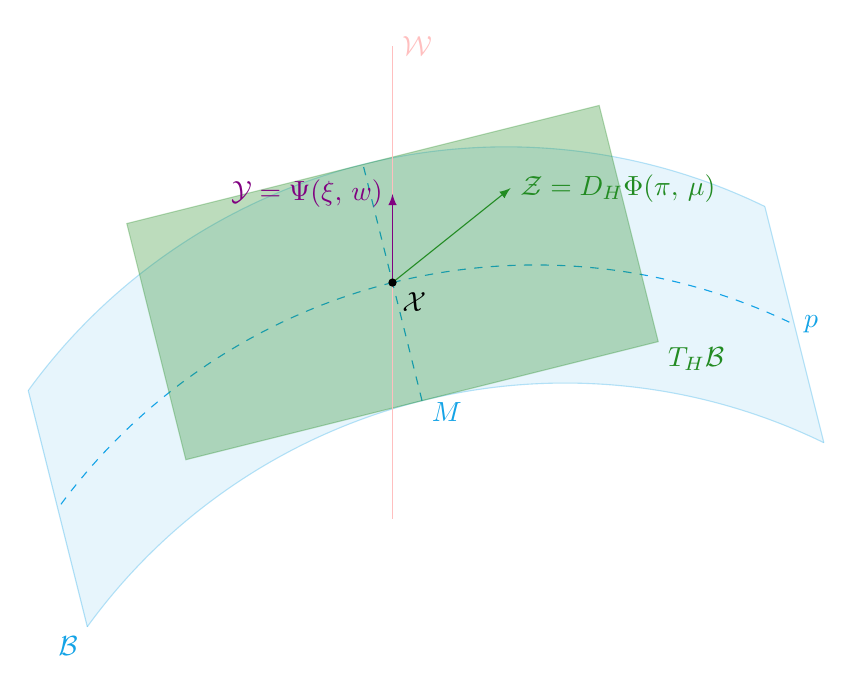
\begin{tikzpicture}[scale=1.5]
    \def\refx{2}
    \def\refy{-7}
	% --------------------------------------------------
	% MANIFOLD BOUNDARIES -- FIRST PASS: NAMING
	% --------------------------------------------------
	% Bottom boundary of the manifold
	\draw[White, opacity=0.3, name path = ManBotRig] (0.25, -1) arc (104.036:64.036:5);
	\draw[White, opacity=0.3, name path = ManBotLef] (0.25, -1) arc (104.036:144.036:5);
	% Top boundary of the manifold
	\draw[White, opacity=0.3, name path = ManTopRig] (-0.25, 1) arc (104.036:64.036:5);
	\draw[White, opacity=0.3, name path = ManTopLef] (-0.25, 1) arc (104.036:144.036:5);
	% --------------------------------------------------
	% MANIFOLD COLOURING
	% --------------------------------------------------
	\tikzfillbetween[of = ManTopLef and ManBotLef, on layer=bg]{White}
	\tikzfillbetween[of = ManTopRig and ManBotRig, on layer=bg]{White}
	\tikzfillbetween[of = ManTopRig and ManBotRig, on layer=bg]{Cerulean, opacity=0.1}
	\tikzfillbetween[of = ManTopLef and ManBotLef, on layer=bg]{Cerulean, opacity=0.1}
	% --------------------------------------------------
	% MANIFOLD BOUNDARIES -- SECOND PASS: SUPERIMPOSED DRAWING
	% --------------------------------------------------
	% Bottom boundary of the manifold
	\draw[Cerulean, opacity=0.3] (0.25, -1) arc (104.036:64.036:5);
	\draw[Cerulean, opacity=0.3] (0.25, -1) arc (104.036:144.036:5);
	% Top boundary of the manifold
	\draw[Cerulean, opacity=0.3] (-0.25, 1) arc (104.036:64.036:5);
	\draw[Cerulean, opacity=0.3] (-0.25, 1) arc (104.036:144.036:5);
	% Right boundary of the manifold
	\draw[Cerulean, opacity=0.3] (3.152, 0.645) -- (3.652, -1.355);
	% Left boundary of the manifold
	\draw[Cerulean, opacity=0.3] (-2.584, -2.914) -- (-3.084, -0.914);
	% Manifold label
	\node[Cerulean, below left] at (-2.584, -2.914) {$\mathcal{B}$};
	% --------------------------------------------------
	% COORDINATES
	% --------------------------------------------------
	% Coordinate p
	\draw[Cerulean, dashed] (0, 0) arc (104.036:64.036:5);
	\draw[Cerulean, dashed] (0, 0) arc (104.036:144.036:5);
	\node[Cerulean, right] at (3.402, -0.355) {$p$};
	% Coordinate M
	\draw[Cerulean, dashed] (0.25, -1) -- (-0.25, 1);
	\node[Cerulean, right] at (0.25, -1-0.1) {$M$};
	% --------------------------------------------------
	% TANGENT SPACE -- SUPERIMPOSED DRAWING
	% --------------------------------------------------
	\draw[color=ForestGreen, fill=ForestGreen, opacity=0.3] (1.75, 1.5) -- (2.25, -0.5) -- (-1.75, -1.5) -- (-2.25, 0.5) -- cycle;
	\node[ForestGreen, right] at (2.25, -0.5-0.15) {$T_H \mathcal{B}$};
	% --------------------------------------------------
	% TANGENT VECTOR
	% --------------------------------------------------
	\draw[ForestGreen, -latex] (0, 0) --	(1, 0.8);
	\node[ForestGreen, right] at		(1, 0.8) {$\mathcal{Z} = D_H \Phi (\pi,\,\mu)$};
	% --------------------------------------------------
	% WAVE SET
	% --------------------------------------------------
	\draw[pink] (0, -2) -- (0, 2);
	\node[pink, right] at (0, 2) {$\mathcal{W}$};
	\draw[Purple, -latex] (0, 0) -- (0, 0.75);
	\node[Purple, left] at (0, 0.75) {$\mathcal{Y} = \Psi (\xi,\,w)$};
	% --------------------------------------------------
	% POINT
	% --------------------------------------------------
	\filldraw (0, 0) circle (0.03);
	\node[below right] at (0,0) {$\mathcal{X}$};
\end{tikzpicture}

\end{document}